\documentclass[a4paper,12pt]{article}



%%% Работа с русским языком
% кодировка
\usepackage[utf8]{inputenc} 
\usepackage[T2A]{fontenc}	
\usepackage[english,russian]{babel}   %% загружает пакет многоязыковой вёрстки
\usepackage{cmap}
\usepackage{algorithm}
\usepackage{algorithmic} 
\usepackage{indentfirst}
\usepackage{xcolor}
\usepackage{hyperref}

% Цвета для гиперссылок
\definecolor{linkcolor}{HTML}{799B03} % цвет ссылок
\definecolor{urlcolor}{HTML}{799B03} % цвет гиперссылок

\hypersetup{pdfstartview=FitH,  linkcolor=linkcolor,urlcolor=urlcolor, colorlinks=true}
%%% Дополнительная работа с математикой
\usepackage{amsmath,amsfonts,amssymb,amsthm,mathtools} % AMS
\usepackage{amsfonts}
\usepackage[miktex]{gnuplottex} % <- Use instead if running TeX Live.

\usepackage{icomma} % "Умная" запятая: $0,2$ --- число, $0, 2$ --- перечисление
%% Номера формул
%\mathtoolsset{showonlyrefs=true} % Показывать номера только у тех формул, на которые есть \eqref{} в тексте.
%\usepackage{leqno} % Нумерация формул слева

%% Свои команды
\DeclareMathOperator{\sgn}{\mathop{sgn}}

%% Перенос знаков в формулах (по Львовскому)
\newcommand*{\hm}[1]{#1\nobreak\discretionary{}
	{\hbox{$\mathsurround=0pt #1$}}{}}

%%% Работа с картинками
\usepackage{graphicx}  % Для вставки рисунков
\usepackage{calc}
\usepackage{subcaption}
\graphicspath{{images/}{images2/}}  % папки с картинками
\setlength\fboxsep{3pt} % Отступ рамки \fbox{} от рисунка
\setlength\fboxrule{1pt} % Толщина линий рамки \fbox{}
\usepackage{wrapfig} % Обтекание рисунков текстом

%%% Работа с таблицами
\usepackage{array,tabularx,tabulary,booktabs} % Дополнительная работа с таблицами
\usepackage{longtable}  % Длинные таблицы
\usepackage{multirow} % Слияние строк в таблице

%%% Теоремы
\theoremstyle{plain} % Это стиль по умолчанию, его можно не переопределять.
\newtheorem{theorem}{Теорема}[section]
\newtheorem{proposition}[theorem]{Утверждение}
\newtheorem{problem}{Задача}[section]

\theoremstyle{definition} % "Определение"
\newtheorem{lemma}{Лемма}[section]
\newtheorem{conclusion}{Следствие}[theorem]

\theoremstyle{remark} % "Примечание"
\newtheorem*{nonum}{Определение}

%%% Программирование
\usepackage{etoolbox} % логические операторы

%%% Страница
\usepackage{geometry} % Простой способ задавать поля
\geometry{top=30mm}
\geometry{bottom=40mm}
\geometry{left=20mm}
\geometry{right=20mm}

%\usepackage{fancyhdr} % Колонтитулы
% 	\pagestyle{fancy}
%\renewcommand{\headrulewidth}{0pt}  % Толщина линейки, отчеркивающей верхний колонтитул
% 	\lfoot{Нижний левый}
% 	\rfoot{Нижний правый}
% 	\rhead{Верхний правый}
% 	\chead{Верхний в центре}
% 	\lhead{Верхний левый}
%	\cfoot{Нижний в центре} % По умолчанию здесь номер страницы
\usepackage[normalem]{ulem}  % для зачекивания текста
\usepackage{setspace} % Интерлиньяж
\onehalfspacing % Интерлиньяж 1.5
%\doublespacing % Интерлиньяж 2

\usepackage{tikz}
\usetikzlibrary{arrows}
\usepackage{lastpage} % Узнать, сколько всего страниц в документе.
\usepackage{soul} % Модификаторы начертания

\usepackage{color}
\usepackage{colortbl}
\usepackage{upgreek}
\usepackage{hyperref}
\usepackage{amsmath,amsfonts,amsthm,amssymb,amsbsy,amstext,amscd,amsxtra,multicol}
\usepackage{indentfirst}
\usepackage{verbatim}
\usepackage{tikz} %Рисование автоматов
\usetikzlibrary{automata,positioning}
\usepackage{multicol} %Несколько колонок
\usepackage{graphicx}
%% \voffset-5mm
%% \def\baselinestretch{1.44}
\renewcommand{\theequation}{\arabic{equation}}
\def\hm#1{#1\nobreak\discretionary{}{\hbox{$#1$}}{}}
\newtheorem{Lemma}{Лемма}
\newtheorem{Remark}{Замечание}
%%\newtheorem{Def}{Определение}
\newtheorem{Claim}{Утверждение}
\newtheorem{Cor}{Следствие}
\newtheorem{Theorem}{Теорема}
\theoremstyle{definition}
\newtheorem{Example}{Пример}
\newtheorem*{known}{Теорема}
\def\proofname{Доказательство}
\theoremstyle{definition}
\newtheorem{Def}{Определение}

%% \newenvironment{Example} % имя окружения
%% {\par\noindent{\bf Пример.}} % команды для \begin
%% {\hfill$\scriptstyle\qed$} % команды для \end


%\date{22 июня 2011 г.}
\let\leq\leqslant
\let\geq\geqslant
\def\MT{\mathrm{MT}}
%Обозначения ``ажуром''
\def\BB{\mathbb B}
\def\CC{\mathbb C}
\def\RR{\mathbb R}
\def\SS{\mathbb S}
\def\ZZ{\mathbb Z}
\def\NN{\mathbb N}
\def\FF{\mathbb F}
%греческие буквы
\let\epsilon\varepsilon
\let\es\emptyset
\let\eps\varepsilon
\let\al\alpha
\let\sg\sigma
\let\ga\gamma
\let\ph\varphi
\let\om\omega
\let\ld\lambda
\let\Ld\Lambda
\let\vk\varkappa
\let\Om\Omega
\def\abstractname{}

\def\R{{\cal R}}
\def\A{{\cal A}}
\def\B{{\cal B}}
\def\C{{\cal C}}
\def\D{{\cal D}}
\let\w\omega

%классы сложности
\def\REG{{\mathsf{REG}}}
\def\CFL{{\mathsf{CFL}}}
\newcounter{uproblem}
\newcounter{subproblem}
\def\pr{\medskip\noindent\stepcounter{problem}{\bf \theproblem .  }\setcounter{subproblem}{0} }
\def\prp{\medskip\noindent\stepcounter{problem}{\bf Задача \theproblem .  }\setcounter{subproblem}{0} }
\def\prstar{\medskip\noindent\stepcounter{problem}{\bf Задача $\theproblem^*$ .  }\setcounter{subproblem}{0} }
\def\prdag{\medskip\noindent\stepcounter{problem}{\bf Задача $\theproblem^\dagger$ .  }\setcounter{subproblem}{0} }
\def\upr{\medskip\noindent\stepcounter{uproblem}{\bf Упражнение \theuproblem .  }\setcounter{subproblem}{0} }
%\def\prp{\vspace{5pt}\stepcounter{problem}{\bf Задача \theproblem .  } }
%\def\prs{\vspace{5pt}\stepcounter{problem}{\bf \theproblem .*   }
\def\prsub{\medskip\noindent\stepcounter{subproblem}{\rm \thesubproblem .  } }
%прочее
\def\quotient{\backslash\negthickspace\sim}
\usepackage{csquotes} % Еще инструменты для ссылок
\usepackage{listings}

\newcolumntype{g}{>{\columncolor{Gray}}c}
\newcolumntype{d}{>{\columncolor{darkishgreen}}c}

\author{
	Ефремов С.В., Якушев А.Ю.}
\title{Методы зеркальных отображений в задачах выпуклой оптимизации}
\begin{document}
	\maketitle
	
	
	\section{Введение}
	Метод зеркального спуска является естественным обобщением метода проекции субградиента в случае обобщения $l_2$ нормы на более общий случай какой-то функции расстояния. В этой работе мы представляем новый подход к построению субградиентной схемы для различных негладких задач выпуклой структуры. Так мы не ограничиваемся построением стандартного метода зеркального спуска, но рассматриваем его вариацию --- метод двойственных усреднений, ускоряем алгоритмы методом подобных треугольников, попутно изучая вопрос выбора констант для его оптимальной работы.
	\section{Постановка задачи}
	
	
	
	Рассмотрим следующую задачу выпуклой оптимизации $-$ задана функция $f(x)$ и оракул также выдает ее градиент $\nabla f(x)$. Задача найти $\min_{x\in \RR} f(x)$.
	
	\subsection{Сопряженная норма:}
	
	\textit{Определение:} Сопряженной нормой $\|\cdot\|_*$ к данной $\|\cdot\|$ называется:
$$
\|y\|_* = \max \{\langle y,x\rangle: \|x\|=1 \}
$$

Пример: $(\|\cdot \|_p)_* = \|\cdot \|_q, \qquad \dfrac{1}{p} + \dfrac{1}{q} = 1$

Неравенство Гельдера:

$$
\sum_{k=1}^n |x_k\,y_k| \le \biggl( \sum_{k=1}^n |x_k|^p \biggr)^{\frac{1}{p}} \biggl( \sum_{k=1}^n |y_k|^q \biggr)^{\frac{1}{q}}
\text{ for all }x, y \in \mathbb{C}^n
$$

Свойства:
\begin{itemize}
\item Двойственная норма $\|\cdot\|_*$ является нормой
\item $l_2$ норма сопряжена сама себе
\item Двойственная норма к двойственной норме - исходная норма
\item $(\|\cdot\|_1)_* = \|\cdot\|_\infty, \;(\|\cdot\|_\infty)_* = \|\cdot\|_1$
\item Обобщенное неравенство Коши Шварца: $\langle y,x \rangle \leq \|y\|_*\|x\|$, следствие: $\|x\|^2 \pm 2 \langle y,x \rangle + \|y\|_*^2 \geq 0$
\end{itemize}

\subsection{Дивергенция (расстояние) Брэгмана}

Попробуем интуитивно ввести понятие обобщенного расстояния, именуемого расстоянием Брэгмана. Для каждой точки $y$ она возвращает расстояние этой точки до $x$ - $V_x(y)$. В самом простом случае можно взять $V_x(y) = \frac{1}{2}\|x-y\|^2, \;\; \nabla V_x(y) = y-x$. Рассмотрим уже классическую запись:

\begin{align*}
\|x_{k+1} - y\|^2  &= \|x_{k+1}-x_k \|^2 + \|x_k - y\|^2 - 2 \langle x_k - x_{k+1} ,x_k - y\rangle \\
V_{x_{k+1}}(y) &= V_{x_{k+1}}(x_k) + V_{x_{k}}(y) - \langle \nabla V_{x_{k+1}(x_k)}, x_k - y \rangle
\end{align*}

Для вводимого обобщенного расстояния будем требовать выполнения, кроме того (как будет видно при получении оценок), приятным свойством было бы еще следующее требование:

$$
V_x(y) \geq \frac{1}{2} \|x-y\|^2
$$

\textit{Определение:} Дивергенцией (расстоянием) Брэгмана называется функция следующая $V_x(y)$. Пусть $S \subseteq \mathbb{R}^n$ - замкнутое выпуклое множество, тогда функция $\phi : S \to \mathbb{R}$ называется прокс-функцией (distance generating function), если $\phi$ является $1$ - сильно выпуклой, т.е.:

$$
\phi(y) \geq \phi(x) + \langle \nabla \phi(x), y-x\rangle + \frac{1}{2} \|y-x\|^2, \qquad \forall x,y \in S
$$

Тогда прокс-функцией индуцируется \textbf{расстояние Брэгмана}:

$$
V_x(y) = \phi(y) - \phi(x) - \langle\nabla \phi(x), y-x\rangle
$$

Заметим, что определение сильной выпуклости зависит от выбора прямой нормы $\|\cdot\|$. Это важное замечание, посольку именно это свойство позволит в будущем подстраивать расстояние под геометрию пространства.

Свойства:
\begin{itemize}
\item Аксиома тождества $V_x(x) = 0$
\item Совместимость с Евклидовой нормой: $V_x(y) \geq \frac{1}{2}\|x-y\|^2 \geq 0$
\item (Не)равенство треугольника: $\langle -\nabla V_x(y), y-z\rangle = V_x(z) - V_y(z) - V_x(y)$
\end{itemize}

\subsection{Вернемся к задаче}

Пусть задано выпуклое замкнутое множество $S \in \mathbb{R}^n$, кроме того, есть алгоритм оптимизации, возвращающий последовательность точек $x_1, \ldots, x_k, \ldots$. Тогда запишем (не)равенство треугольника для расстояния Брэгмана, полагая $y = x_{k+1}, x = x_k$ и произвольный $z \in S$ (который мы в дальнейшем для целостности изложения будем обозначать $y$)

\begin{align*}
\langle -\nabla V_{x_k}(x_{k+1}), x_{k+1}-z\rangle &= V_{x_k}(z) - V_{x_{k+1}}(z) - V_{x_k}(x_{k+1}) \\
\tag{baseMD}
\langle -\nabla V_{x_k}(x_{k+1}), x_{k+1}-y\rangle &= V_{x_k}(y) - V_{x_{k+1}}(y) - V_{x_k}(x_{k+1})
\end{align*}

Просуммируем полученные равенства:

$$
\sum\limits_{k = 0}^{T-1}\langle -\nabla V_{x_k}(x_{k+1}), x_{k+1}-y\rangle = V_{x_0}(y) - V_{x_{T}}(y) - \sum\limits_{k = 0}^{T-1}V_{x_k}(x_{k+1})
$$

Имея ввиду полученное уравнение, давайте, наконец, попробуем сформулировать метод \textbf{зеркального спуска}:

$$
x_{k+1} = \text{arg}\min\limits_{x \in S} \left( \langle \alpha_k g_k, x \rangle + V_{x_k}(x) \right)
$$

Посмотрим внимательнее на условие проекции для точки $x_{k+1}$:

$$
\langle \alpha_k g_k,x_{k+1} - y\rangle + \langle \nabla V_{x_k}(x_{k+1}),x_{k+1} - y\rangle \leq 0
$$

$$
\langle \alpha_k g_k,x_{k+1} - y\rangle \leq - \langle \nabla V_{x_k}(x_{k+1}),x_{k+1} - y\rangle 
$$

Попробуем теперь получить наше базовое неравенство, используя (baseMD):
\begin{align*}
\langle \alpha_k g_k, x_k - y\rangle &\leq - \langle \nabla V_{x_k}(x_{k+1}),x_{k+1} - y\rangle - \langle \alpha_k g_k, x_{k+1} - x_k\rangle = \\
& = V_{x_k}(y) - V_{x_{k+1}}(y) - V_{x_k}(x_{k+1})- \langle \alpha_k g_k, x_{k+1} - x_k\rangle \leq\\
&\leq V_{x_k}(y) - V_{x_{k+1}}(y) - \frac{1}{2}\|x_k - x_{k+1}\|^2- \langle \alpha_k g_k, x_{k+1} - x_k\rangle \leq \\
&\leq V_{x_k}(y) - V_{x_{k+1}}(y) + \left(\langle \alpha_k g_k, x_k - x_{k+1}\rangle- \frac{1}{2}\|x_k - x_{k+1}\|^2 \right) \leq \\
&\leq V_{x_k}(y) - V_{x_{k+1}}(y) + \frac{\alpha_k^2}{2} \|g_k\|_*^2
\end{align*}

ТЕЛЕСКОПИРУЕМ

\begin{align*}
\sum\limits_{k = 0}^{T-1} \langle \alpha_k g_k, x_k - y\rangle &\leq  V_{x_0}(y) - V_{x_{T}}(y) + \sum\limits_{k = 0}^{T-1}\frac{\alpha_k^2}{2} \|g_k\|_*^2 \\
&\leq V_{x_0}(y)  + \sum\limits_{k = 0}^{T-1}\frac{\alpha_k^2}{2} \|g_k\|_*^2 \\
&\leq M + \dfrac{\alpha^2 G^2 T}{2} 
\end{align*}

Здесь мы подразумеваем $\|g_k\|_* \leq G$ равномерно по $k$, а $V_{x_0}(y) \leq M$. В итоге:

\begin{align*}
f(\overline{x}) - f^* &= f \left( \frac{1}{T}\sum\limits_{k=0}^{T-1} x_k \right) - f^* \leq \dfrac{1}{T} \left( \sum\limits_{k=0}^{T-1} f(x_k) - f^* \right) \\
& \leq  \dfrac{1}{T} \left( \sum\limits_{k=0}^{T-1}\langle g_k, x_k - x^* \rangle\right) \\
& \leq \dfrac{M}{\alpha T} + \dfrac{\alpha G^2}{2} \leq \sqrt{\dfrac{2 M G^2}{T}}
\end{align*}

Выбирая шаг $\alpha_k = \alpha = \sqrt{\dfrac{2M}{G^2 T}}$

\subsection{Алгоритм зеркального спуска (mirror descent):}
$$
x_{k+1} = \text{arg}\min\limits_{x \in S} \left( \langle \alpha_k g_k, x \rangle + V_{x_k}(x) \right)
$$

Интересные фишки:
\begin{itemize}
    \item Такая же скорость сходимости, как и для метода проекции субградиента.
    \item Работает в существенно более широком классе практических задач.
\end{itemize}

\subsection{Ценность}

В случае, если мы выбрали $\|\cdot\| = \|\cdot\|_2$ Евклидову норму и Евклидово расстояние, то этот метод в точности совпадает с тем, что мы уже называем метод проекции субградиента. 

Значит, надо предоставить сценарий, когда МЗС работает лучше, давайте рассмотрим $S = \Delta_n$ - вероятностный симплекс, а так же следующее расстояние Брэгмана $V_x(y) = \sum_{i \in [n]} y_i \log \frac{y_i}{x_i} = D(y \| x)$. Норма в прямом пространстве при этом $\|\|_1$, а в сопряженном - $\|\|_\infty$. Кроме того, для заданной дивергенции Брэгмана справедливо:
$$
x_0 = \left( 1/n, \ldots, 1/n \right) \; \to \; V_{x_0}(x) \leq \log n \;\;\forall x \in \Delta_n
$$

Тогда алгоритм зеркального спуска запишется в виде:

\begin{align*}
x_{k+1} &= \text{arg}\min\limits_{x \in S} \left( \langle \alpha_k g_k, x \rangle + V_{x_k}(x) \right) \\
&= \text{arg}\min\limits_{x \in S} \left( \langle \alpha_k g_k, x \rangle + \sum_{i \in [n]} x_i \log \frac{x_i}{x_{k_i}} \right) \\
&= x_k \cdot \dfrac{e^{-\alpha_k g_k}}{\|x_k \cdot e^{-\alpha_k g_k}\|_1}
\end{align*}

А оценки с учетом того, что $M = \log n, \|g_k\|_\infty \leq G$ запишутся, как:
\begin{align*}
f(\overline{x}) - f^*  \leq \sqrt{\dfrac{2 \log (n) G^2}{T}}
\end{align*}
	
Таким образом, получаем алгоритм зеркального спуска:
	
	\begin{algorithm}[h!]
		\caption{Mirror Descent}
		\hspace*{\algorithmicindent} \textbf{Input}: $x_0, f(x), \nabla f(x), \alpha$
		\begin{algorithmic}[1]
			\FOR  {$k=0,1,\dots,K$}
			\STATE {$x_{k+1} = \text{arg}\min\limits_{x \in S} \left( \langle \alpha_k g_k, x \rangle + V_{x_k}(x) \right)$}
			\ENDFOR
		\end{algorithmic}
		\textbf{Output}: ${x}_{K+1}$
	\end{algorithm}
	
	
	\newpage	
	\section{Описание методов}
	\subsection{Двойственные усреднения}
	Предлагается исследовать также метод двойственных усреднений. В общем виде:
	
	\begin{algorithm}[h!]
		\caption{Dual Averaging}
		\textbf{Input}: Set $s_0=0$,Choose $\beta_0>0$.
		\begin{algorithmic}[1]
			\FOR  {$k=0,1,\dots,K$}
			\STATE {Compute $g_k= \nabla f(x_k)$}
			\STATE {Choose $\lambda_k > 0$. Set $s_{k+1} = s_k + \lambda_k g_k$}
			\STATE {Choose $\beta_{k+1}\geqslant \beta_k$. Set $x_{k+1}=\pi_{\beta_{k+1}}(-s_{k+1})$.}
			\ENDFOR
		\end{algorithmic}
	\end{algorithm}
	
	Где $\pi_{\beta}(s) = \text{arg}\min\limits_{x \in Q}(-\langle s, x\rangle + \beta d(x))$, причем $d(x)= \sum\limits_{i}x_i \log x_i$.
	
    Тогда, получаем:
    
\begin{align*}
\text{arg}\min\limits_{x \in Q}(-\langle s, x\rangle + \beta \sum\limits_{i}x_i \log x_i)\\
=\text{arg}\min(\langle \frac{-s}{\beta}, x\rangle + \sum\limits_{i}x_i \log \frac{x_i}{x_0} + \sum\limits_{i}x_i \log x_0)\\
=\text{arg}\min(\langle \frac{-s}{\beta}, x\rangle + \sum\limits_{i}x_i \log \frac{x_i}{x_0} - \sum\limits_{i}x_i \log n)\\
=\text{arg}\min(\langle \frac{-s}{\beta}, x\rangle + \sum\limits_{i}x_i \log \frac{x_i}{x_0} - \log n)\\
=\text{arg}\min(\langle \frac{-s}{\beta}, x\rangle + \sum\limits_{i}x_i \log \frac{x_i}{x_0}\\
=x_0\cdot \frac{e^{\frac{s}{b}}}{\|x_0\cdot e^{\frac{s}{b}}\|}\\
=\frac{e^{\frac{s}{b}}}{\|e^{\frac{s}{b}}\|} 
\end{align*}
	
А значит, можно выразить $x_{k+1} = x_k\cdot \frac{e^{-g_k\alpha}}{\|x_k e^{-g_k\alpha}\|}$.	
    \subsection{Метод подобных треугольников}	
Заметим, что оба, описанных выше метода могут быть ускорены с помощью метода подобных треугольников.

\begin{algorithm}[h!]
		\caption{Similar Triangles}

		\begin{algorithmic}
			\STATE {$y_{k+1}=\frac{\alpha_{k+1} u_k + A_k x_k}{A_{k+1}}$}
			\STATE {$u_{k+1}=\text{arg}\min\limits_{x \in Q}\varphi_{k+1}(x)$}
			\STATE {$x_{k+1}=\frac{\alpha_{k+1} u_{k+1} + A_k x_k}{A_{k+1}}$}
			\STATE {$A_k = \sum\limits_{i=0}^{k} \alpha_i, \alpha_0 = L^{-1}, x_0=u_0=\text{arg}\min\limits_{x \in Q}\varphi_0(x)$}
		\end{algorithmic}
	\end{algorithm}
	
	Где $\alpha_{k+1}$ можно задавать рекуррентно:
	$$
	\alpha_{k+1}=\frac{1}{2L}+\sqrt{\frac{1}{4L^2}+\alpha_k^2},
	$$
	
	и тогда мы получим еще 2 метода TR-MD и TR-DA.
	
	Но можно подойти к выбору $\alpha_k$ чуть более нестандартно.
	
	Возьмем:
	
	$$
	\alpha_k = \text{arg}\min\limits_{\alpha_k \in M}(f(y_k))=\text{arg}\min\limits_{\alpha_k \in M}f(\alpha_{k+1} u_k + (1-\alpha_{k+1}) x_k)
	$$
	
	Таким образом вывели еще два оптимизированных методом подобных треугольников, но для других альфа алгоритма TR-MD2 и TR-DA2.
	
	\section{Эксперименты}
	
	
    В ходе экспериментов мы тестируем работу полученных выше алгоритмов и сравниваем скорость их сходимости к точному решению. Для тестирования взяли функцию:
    
    $$
    f(x) = \|Ax - b\|_2^2
    $$
    $$
    \nabla f(x) = 2A^T(Ax-b)
    $$
	
	И будем искать ее минимум на выпуклом множестве $S : \left\{x \in S : x \geq 0, \sum\limits_{i \in [n]} x_i = 1\right\}$ (вероятностном симплексе).
	
	Но для последних 2-x методов знания значений градиента оказывается недостаточно. Необходимо в явном виде выразить $\alpha$.
	
	$$
	\alpha =\text{arg}\min\limits_{\alpha}f(\alpha x^n + (1-\alpha) y^n)
	$$
	$$
	\sum\limits_{k=1}^{n}(x_k^n-y_k^n)\frac{\partial f(\alpha x^n + (1-\alpha) y^n)}{\partial x_k}
	$$
	$$
	(x^n-y^n)^T \nabla f(\alpha x^n + (1-\alpha) y^n)=0
	$$
	$$
	(x^n-y^n)^T 2A^T(A(\alpha x^n + (1-\alpha) y^n)-b)=0
	$$
	$$
	2(x^n-y^n)^T (\alpha (A^T(A x^n -b)) + (1-\alpha)(A^T(A y^n-b)))=0
	$$
	$$
	(x^n-y^n)^T (\alpha \nabla f(x^n)  + (1-\alpha)\nabla f(y^n))=0
	$$
	
\begin{equation*}
\alpha= 
 \begin{cases}
   const = 0 & (x^n-y^n)^T (\nabla f(x^n) - \nabla f(y^n)) = 0\\
   -\frac{(x^n-y^n)^T (\nabla f(y^n))}{(x^n-y^n)^T (\nabla f(x^n) - \nabla f(y^n))} & else
 \end{cases}
\end{equation*}
	
	Полученные результаты представлены на графиках.
  
  \begin{figure}[!htb]
    \minipage{0.5\textwidth}
    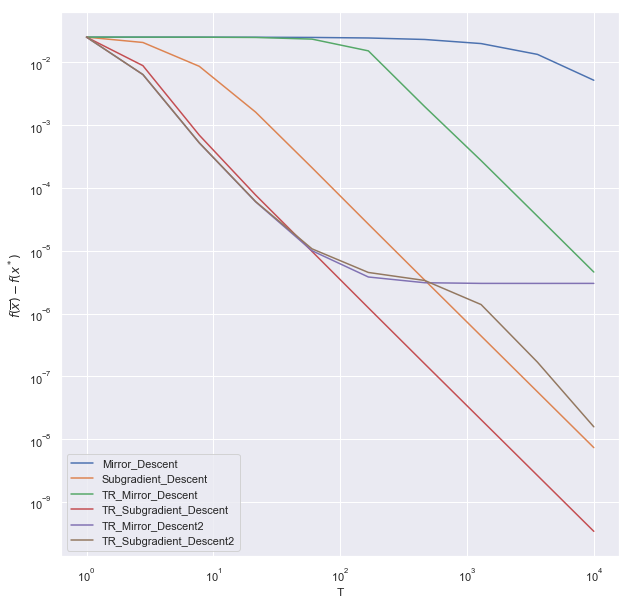
\includegraphics[width=\linewidth]{MD.png}
    \endminipage\hfill
    \minipage{0.5\textwidth}
    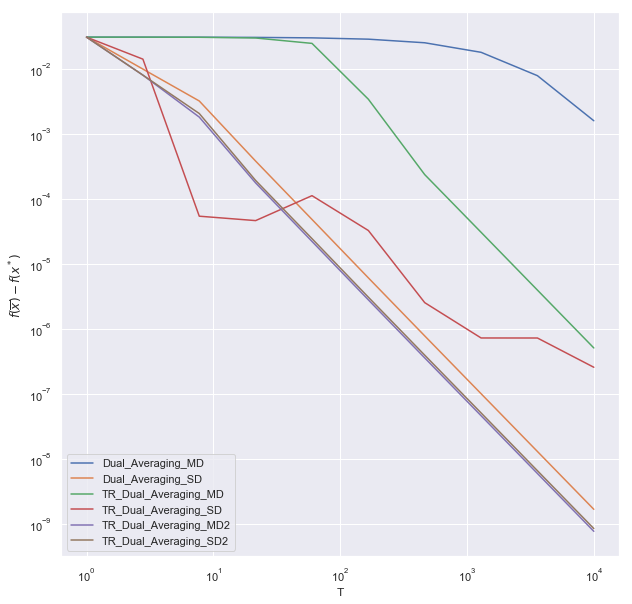
\includegraphics[width=\linewidth]{DA.png}
    \endminipage
    \caption{На левом графике результаты работы для метода зеркального спуска и его ускорений, на правом аналогично для метода двойственных усреднений.}
  \end{figure}

	
	\section{Заключение}
	В данной работе был реализован метод зеркального спуска и рассмотрены различные его вариации. Нетрудно заметить из графиков, что ускорение получается более чем существенное и ускоренные методы сходятся значительно быстрее. Наиболее быстрым оказывается метод двойственных с взвешенными $\lambda$ оптимизированный методом подобных треугольников с особым выбором коэффициента $\alpha$.
	
	\paragraph{Responsibilities:}
	
\begin{itemize}
    \item Code director - Якушев А.Ю.
    \item Text director - Ефремов С.В.
\end{itemize}
	
	\newpage
	
	\begin{thebibliography}{4} 
		\bibitem{gas} \textit{Гасников А.В.} Современные численные методы оптимизации. Метод универсального градиентного спуска
		
		\bibitem{seminar} \textit{Камзолов Д.И.} Семинары 674 группы 
		
		\bibitem{presentation} \textit{Камзолов Д.И.} Презентации 674 группы
		
		\bibitem{nest} \textit{Нестеров Ю.} Primal-dual subgradient methods for convex problems
		
		\bibitem{nest} \textit{Гасников А.В., Нестеров Ю.Е.} Универсальный метод для задач стохастической композитной оптимизации
		
		\bibitem{presentation} \textit{Меркулов Д.} Презентации
		
	\end{thebibliography}
	
	
\end{document} 	